%% abtex2-modelo-slides.tex, v-1.0 gfabinhomat
%% Copyright 2012-2016 by abnTeX2 group at http://www.abntex.net.br/ 
%%
%% This work may be distributed and/or modified under the
%% conditions of the LaTeX Project Public License, either version 1.3
%% of this license or (at your option) any later version.
%% The latest version of this license is in
%%   http://www.latex-project.org/lppl.txt
%% and version 1.3 or later is part of all distributions of LaTeX
%% version 2005/12/01 or later.
%%
%% This work has the LPPL maintenance status `maintained'.
%% 
%% The Current Maintainer of this work is Fábio Rodrigues Silva, 
%% member of abnTeX2 team, led by Lauro César Araujo. 
%% Further information are available on 
%% http://www.abntex.net.br/
%%
%% This work consists of the files abntex2-modelo-slides.tex, 
%% abntex2-modelo-references.bib and abntex2-modelo-marca.pdf
%%
%% Modelo desenvolvido por Fábio Rodrigues Silva (gfabinhomat@gmail.com)
%% Mais informações podem ser obtidas no guia do usuário Beamer 
%% (http://linorg.usp.br/CTAN/macros/latex/contrib/beamer/doc/beameruserguide.pdf)
%% Informações rápidas podem ser acessadas em http://en.wikibooks.org/wiki/LaTeX/Presentations


% Apresentações em widescreen. Outros valores possíveis: 1610, 149, 54, 43 e 32.
% Por padrão, as apresentações são no formato 4:3 (sem o aspectratio).
%\documentclass[aspectratio=169, xcolor=table]{beamer}
\documentclass[aspectratio=169]{beamer}
%[aspectratio=169]
\usetheme{Pittsburgh}
\usecolortheme{default}
\usefonttheme[onlymath]{serif}			% para fontes matemáticas
% Enconte mais temas e cores em http://www.hartwork.org/beamer-theme-matrix/ 
% Veja também http://deic.uab.es/~iblanes/beamer_gallery/index.html

% Customizações de Cores: fg significa cor do texto e bg é cor do fundo
\setbeamercolor{normal text}{fg=black}
\setbeamercolor{alerted text}{fg=red}
\setbeamercolor{author}{fg=blue}
\setbeamercolor{institute}{fg=blue}
\setbeamercolor{date}{fg=green}
\setbeamercolor{frametitle}{fg=red}
\setbeamercolor{framesubtitle}{fg=brown}
\setbeamercolor{block title}{bg=blue, fg=white}		%Cor do título
\setbeamercolor{block body}{bg=gray, fg=darkgray}	%Cor do texto (bg= fundo; fg=texto)

\setbeamertemplate{navigation symbols}{ %\insertslidenavigationsym\\
\insertframenavigationsymbol \insertsubsectionnavigationsymbol \insertsectionnavigationsymbol \insertdocnavigationsymbol \insertbackfindforwardnavigationsymbol \hspace{1em} 	\usebeamerfont{footline}
\insertframenumber/\inserttotalframenumber%
}

% ---
% PACOTES
% ---
\usepackage[alf]{abntex2cite}		% Citações padrão ABNT
\usepackage[english]{babel}		% Idioma do documento
\usepackage{color}			% Controle das cores
\usepackage[T1]{fontenc}		% Selecao de codigos de fonte.
\usepackage{graphicx}			% Inclusão de gráficos
\usepackage[utf8]{inputenc}		% Codificacao do documento (conversão automática dos acentos)
\usepackage{txfonts}			% Fontes virtuais
%\usepackage{listings,bera}
\usepackage[portugues,ruled,lined]{algorithm2e}
\usepackage{algorithmic}
\usepackage{mathtools} % loads amsmath
\usepackage[absolute,overlay]{textpos}
\usepackage{tikz}
\usetikzlibrary{shadows}
%\usepackage[noend]{algpseudocode}
\usepackage{algorithmic}
\setbeamertemplate{caption}[numbered]


\usepackage{listings}
\usepackage{adjustbox}

% ---

% --- Informações do documento ---
\title{Radio Communication to Control and Run an Autonomous Mission for UAVs via a Mobile Application}
\author{Thiago Rodrigo Félix Cavalcante}
%\institute{Programa de Pós-Graduação em Engenharia Elétrica
%	    \par
%	    Faculdade de Tecnologia}
\date{Manaus, \today}
% ---

%**
% \PutAt<overlay spec>[<box width>]{(<x>, <y>)}{<content>}
%
% real absolute positioning of <content> on a slide, if content is a figure,
% minipage or whatever kind of LR-box, the <box width> argument may be omitted
%
%
% implementation notes: 
%   - based on   \usepackage[absolute,overlay]{textpos}
%   - NOT combinable with any beamer feature that is based on pgfpages
%     (such as dual-screen support, built-in 2up handouts, etc.), as textpos 
%     and pgfpates interfere at the shippout-level.
%

  \newcommand<>{\PutAt}[3][0pt]{%
    {\only#4{\begin{textblock*}{#1}#2%
      #3
    \end{textblock*}}}%
  }

%**
% \ShowPutAtGrid
%
% draws a helpful grid on the current slide to figure <x> and <y> parameters for \PutAt
% 
  \newcommand{\ShowPutAtGrid}{
    \begin{textblock*}{128mm}(0cm,0cm)
    \tikz[color=red!20!white]\draw[very thin, step=5mm] (0mm,0mm) grid (130mm,100mm);
    \end{textblock*}
    \begin{textblock*}{128mm}(0cm,0cm)
    \begin{tikzpicture}[color=red]
      \draw[step=1cm] (0,0mm) grid (130mm,100mm);   
      \foreach \n in {0,...,12}
        \draw[xshift=.5mm,yshift=-1.5mm, inner sep=0pt, anchor=west] (\n,10) node {\scriptsize{\textbf{\n}}};
      \foreach \n in {1,...,9}
        \draw[xshift=.5mm,yshift=-1.5mm, inner sep=0pt, anchor=west] (0,10-\n) node {\scriptsize{\textbf{\n}}};
    \end{tikzpicture}
    \end{textblock*}
  }


%**
% \NormalBox<overlay spec>[tikz picture/node options]{<content>}
%
% draws content boxed in a nice box
% 
\newcommand<>{\NormalBox}[2][]{%
  \only#3{\tikz[#1, every node/.style={shape=rectangle,draw,fill=white, drop shadow, #1}]\node []{#2};}
}
%**
% \OrangeBox<overlay spec>[tikz picture/node options]{<content>}
%
% draws content boxed in an orange call-out box
% 
\newcommand<>{\OrangeBox}[2][]{%
  \onslide#3{\NormalBox[fill=orange!30,draw=black!30,rounded corners=4pt,#1]{#2}}%
}


% ----------------- INÍCIO DO DOCUMENTO --------------------------------------
\begin{document}

% ----------------- NOVO SLIDE --------------------------------
\begin{frame}

\begin{minipage}{1\linewidth}
  \centering
  \begin{tabular}{cc}
    \begin{tabular}{c}
      
\includegraphics[scale=0.1]{ufam.eps}
    \end{tabular}
    &
    \begin{tabular}{c}
      \textbf{Universidade Federal do Amazonas} \\ \textbf{Faculdade de Tecnologia}
    \end{tabular}
  \end{tabular}
\end{minipage}

\titlepage

\end{frame}

% ----------------- NOVO SLIDE --------------------------------
\begin{frame}{Contents}
\tableofcontents
\end{frame}


% ----------------- NOVO SLIDE --------------------------------
\section{Program Synthesis}

\begin{frame}{Introduction}

Logistics has become a competitive and fundamental factor for organizations, involving the management, conservation, and supervision of freight transport. In addition, excellent logistics means client satisfaction; so speed is still an important factor in a successful logistics process~\cite{drone4logistic}.


\end{frame}
\begin{frame}{Program Synthesis}

Program Synthesis is the task of discovering an executable program from user intent expressed in the form of some constraints


\end{frame}
\begin{frame}{Program Synthesis}
\frametitle{Program Synthesis}\pause 	
\framesubtitle{Domain specific synthesis}
Domain specific systems take the human insight and build it directly into the synthesizer.\pause

\begin{itemize}
\item AutoBayes - data analysis programs from statistical models;\pause
\item FFTW - produces fast Fourier transforms optimized for 
specic architectures;\pause
\item Generate implementations that often outperform hand-written code;\pause
\item Very specific to a field and rely on domain specific knowledge.
\end{itemize}

\end{frame}

\begin{frame}{Program Synthesis}
\frametitle{Program Synthesis}\pause 	
\framesubtitle{Deductive approach}

\begin{itemize}
\item Synthesis systems which allow the user to provide insight directly into the synthesizer;\pause
\item Program can be extracted from a constructive proof of the satisfiability of a specification – KIDS \cite{smith1990kids}, NuPRL \cite{constable1986implementing};\pause
\item In the hands of experts, these systems are extremely powerful (correct implementation);\pause
\item Demands a high level of expertise.
\end{itemize}

\end{frame}

\begin{frame}{Program Synthesis}
\frametitle{Program Synthesis}\pause 	
\framesubtitle{Sketching}
A form of synthesis that uses partial programs as a communication device between the programmer and the synthesizer.\pause

\begin{itemize}
\item focus the synthesizer on low-level details, leaving control of the high-level strategy in the hands of the programmer.
\end{itemize}

\end{frame}

\begin{frame}{Program Synthesis}
\frametitle{Program Synthesis}\pause
Find a program $P$ that meets a specification $\phi(input, output)$:\pause

\begin{equation}
\exists P \forall x . \phi(x, P(x))
\end{equation}

\end{frame}

\newlength\someheight
\setlength\someheight{3cm}

\begin{frame}[fragile]
    \frametitle{Program Synthesis}\pause
	\framesubtitle{List example}
    \begin{adjustbox}{width=\textwidth,height=\someheight,keepaspectratio}
    \begin{lstlisting}
        list reverse (list l){
            if (isEmpty(l)){
                return l;
            }
            else{
                node n = popHead(l);
                return append(reverse(l), n);
            }
        }
    \end{lstlisting}
    \end{adjustbox}
\end{frame}

\begin{frame}[fragile]
    \frametitle{Program Synthesis}\pause
	\framesubtitle{List example}
    \begin{adjustbox}{width=\textwidth,height=\someheight,keepaspectratio}
    \begin{lstlisting}
        list reverseEfficient(list l){
            list nl = new list();
            while(.){.}
        }
    \end{lstlisting}
    \end{adjustbox}
\end{frame}

\begin{frame}{Program Synthesis}
\frametitle{Program Synthesis}
\framesubtitle{List example}

The condition for the loop must be a pointer comparison involving some of the memory locations reachable from l and nl.

These conditions are stated as expressions called generators.

$\#define ~LOC ~\{ ~|(l ~| ~nl).(head ~| ~tail)(.next)? ~| ~null ~|\}$

$\#define ~COMP ~\{| ~LOC ~( ~== ~| ~!= ~) ~LOC ~|\}$

\end{frame}

\begin{frame}[fragile]
    \frametitle{Program Synthesis}\pause
	\framesubtitle{List example}
    \begin{adjustbox}{width=\textwidth,height=\someheight,keepaspectratio}
    \begin{lstlisting}
        list reverseEfficient(list l){
            #define LOC {|(l | nl).(head | tail)(.next)? | null |} 
            #define COMP {| LOC ( == | != ) LOC |}
            
            list nl = new list();
            while(COMP){.}
        }
    \end{lstlisting}
    \end{adjustbox}
\end{frame}

\begin{frame}{Program Synthesis}
\frametitle{Program Synthesis}\pause 	
\framesubtitle{Deductive approach}

\begin{itemize}
\item A sequence of assignments to some of the available pointers;\pause
\item Guard assignments with some condition;\pause
\item Temporary variable is required;\pause
\item Use a different iteration condition for the first iteration.
\end{itemize}

\end{frame}

\begin{frame}[fragile]
    \frametitle{Program Synthesis}\pause
	\framesubtitle{List example}
    \begin{adjustbox}{width=\textwidth,height=\someheight,keepaspectratio}
    \begin{lstlisting}
    	#define LOC {|(l | nl).(head | tail)(.next)? | null |} 
        #define COMP {| LOC ( == | != ) LOC |}
        list reverseEfficient(list l){
            list nl = new list();
            node tmp = null;
            bit c = COMP;
            while(c){
            	if( COMP ){ LHS = LOC2; }
            	if( COMP ){ LHS = LOC2; }
            	if( COMP ){ LHS = LOC2; }
            	if( COMP ){ LHS = LOC2; }
            	if( COMP ){ LHS = LOC2; }
            	c = COMP;
            }
         }
    \end{lstlisting}
    \end{adjustbox}
\end{frame}

\begin{frame}{Program Synthesis}
\frametitle{Program Synthesis}\pause
Find a program $P$ that meets a specification $\phi(input, output)$:\pause

\begin{equation}
\exists P \forall x . \phi(x, P(x))
\end{equation}

\end{frame}

\begin{frame}[fragile]
    \frametitle{Program Synthesis}\pause
	\framesubtitle{List example}
    \begin{adjustbox}{width=\textwidth,height=\someheight,keepaspectratio}
    \begin{lstlisting}
    	main(bit [N] elems, int n){
            if( n < N){
            	list l1 = populate(elems, n);
            	list l2 = populate(elems, n);
            	l1 = reverse(l1);
            	l2 = reverseEfficient(l2);
            	assert compare(l1, l2);
            }
       }
    \end{lstlisting}
    \end{adjustbox}
\end{frame}

\begin{frame}{Program Synthesis}
\frametitle{Program Synthesis}\pause
\framesubtitle{Counterexample Guided Inductive Synthesis (CEGIS)}

In sketching, user insight is provided in the form of a partial program that needs to be completed.\pause

Synthesis problem is reduced to a search for constant values to assign to each hole in the sketch.

\end{frame}

\begin{frame}{Program Synthesis}
\frametitle{Program Synthesis}
\framesubtitle{Counterexample Guided Inductive Synthesis (CEGIS)}

 \begin{figure}[H]
  \centering
  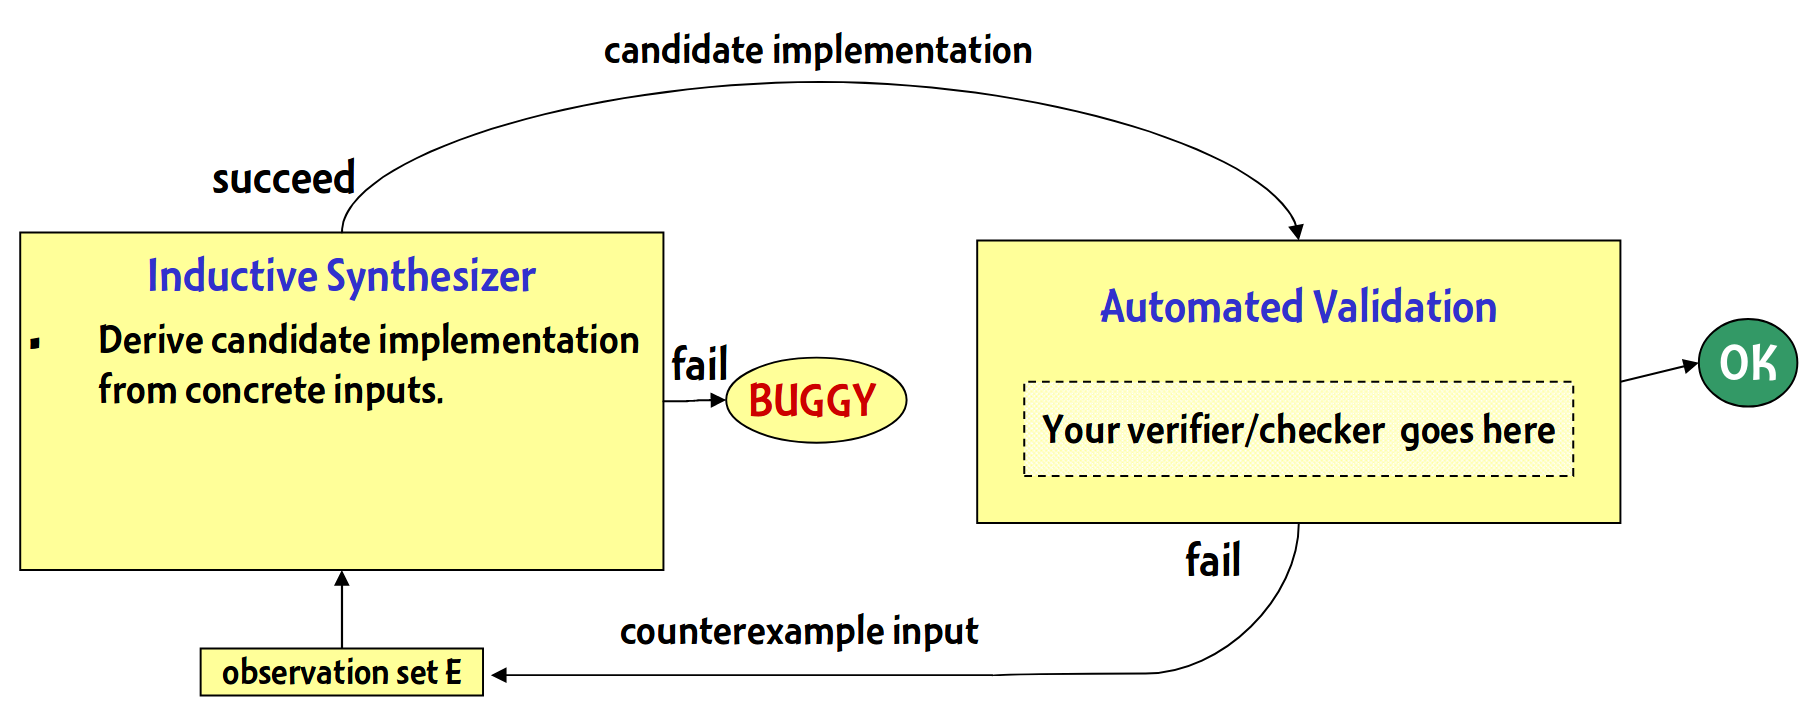
\includegraphics[scale=0.2]{diagram1.png}
  \caption{Counterexample driven synthesis algorithm. Source: \url{https://www2.eecs.berkeley.edu/Pubs/TechRpts/2008/EECS-2008-177.html}}
\end{figure}

\end{frame}

\begin{frame}{Program Synthesis}
\frametitle{Program Synthesis}
\framesubtitle{Counterexample Guided Inductive Synthesis (CEGIS)}

\begin{itemize}
\item The inductive synthesizer uses each new 
observation to refine its hypothesis about 
what the correct program should be until it 
converges to a solution;\pause
\item Validation procedure checks the candidate 
implementation produced by the inductive 
synthesizer;\pause
\item Validation procedure is expected to produce 
a concrete input which exhibits the bug in 
the candidate program.
\end{itemize}

\end{frame}

\section{Paper Progress}
\begin{frame}{Paper Progress}
\frametitle{Paper Progress}
\framesubtitle{Digital Control Systems - Math Proof}

\begin{itemize}
\item Modelling of an expression to verify that a settling time given by the synthesizer satisfies the settling time required;\pause\item Implementing the checker in C;\pause
\item Needs to be fined and validated.
\end{itemize}

\end{frame}

\begin{frame}{Paper Progress}
\frametitle{Paper Progress}
\framesubtitle{Digital Control Systems - Math Proof}

\emph{Modelling}:

The output of a Discrete System can be given by:
\begin{equation}
y[k]=CA^kx[0]+\sum_{m=0}^{k-1}(CA^{k-m-1}Bu[m])+Du[k]
\end{equation}
or by:
\begin{equation}
y[k]=y_{ss}+\sum_{i=1}^{n}C_i\lambda_i^k
\end{equation}

Modelled expression to prove the satisfiability:
\begin{equation}\label{eq:saidaNova}
\overline{y}[k]=y_{ss}+n\overline{C}\overline{\lambda}^k
\end{equation}


\end{frame}

\definecolor{keywords}{RGB}{255,0,90}
\definecolor{comments}{RGB}{60,179,113}
\lstset{language=C,
keywordstyle=\color{keywords},
commentstyle=\color{comments}\emph}
\begin{frame}[fragile]
\frametitle{Paper Progress}
\framesubtitle{Implementation of the checker in C}\pause

\emph{Procedures}:
\begin{lstlisting}
complex double *getEigvalues(MAT *A);
double maxMagEigVal(complex double *z, size_t size);
double log_b(double base, double x);
double k_ss(MAT *A, MAT *B, MAT *C, MAT *D, double p, double u);
\end{lstlisting}

\end{frame}

% ----------------- NOVO SLIDE --------------------------------
\section{References}

% --- O comando \allowframebreaks ---
% Se o conteúdo não se encaixa em um quadro, a opção allowframebreaks instrui 
% beamer para quebrá-lo automaticamente entre dois ou mais quadros,
% mantendo o frametitle do primeiro quadro (dado como argumento) e acrescentando 
% um número romano ou algo parecido na continuação.

\begin{frame}[allowframebreaks]{References}
\bibliography{ref-slides}
\end{frame}

% ----------------- FIM DO DOCUMENTO -----------------------------------------
\end{document}
